\documentclass{beamer}
\usepackage[utf8]{inputenc}

\usetheme{Madrid}
\usecolortheme{beaver}
\usepackage{charter}
\usepackage{tikz}
\usepackage{graphicx}
\usepackage{amsmath}
\usepackage{amssymb}
\usepackage{pgfplots}
\pgfplotsset{width=5.6cm,compat=1.7}

\pgfdeclareimage[width=\paperwidth]{title}{images/oill.jpg}
\setbeamerfont{subtitle}{size=\tiny}
\setbeamertemplate{title page}{
    \begin{picture}(0,0)
        \put(-20.5,-140){%
            \pgfuseimage{title}
        }
        \put(0,-105){%
            \begin{minipage}[b][4.5cm][t]{0.5\textwidth}
                \color{black}
                \usebeamerfont{title}
                    {\inserttitle\\[0.9cm]}
                \usebeamerfont{subtitle}
                    {\insertauthor\par}
                    {\insertinstitute\\[0.3cm]}
                    {\insertdate}
            \end{minipage}
        }
    \end{picture}
}



\title[CBD super]{Friends With Benefits:   Skincare and CBD} 
\author%
{%
    \sc{E.Kurlovich}\\
    \textit{Scientist}
}
\institute%
{%
    \textit{Beauty institute}\\
    \textit{University of Oxford}
}
\date[2022]{Presentation on CBD in skincare, July 2022} % short date for footer



\begin{document}
    \begin{frame}[plain]
        \titlepage
    \end{frame}
    
    \begin{frame}
       
        \frametitle{What is CBD?}
        \framesubtitle{A bit more information about this}
        
        CBD  – a natural compound found in cannabis plants. These plants contain two primary active ingredients: THC and CBD. THC is the psychoactive ingredient while CBD isn’t. CBD pumps you up with antioxidants and alleviate anxiety and inflammation. It is used as an epilepsy treatment and it’s linked to pain relief.
        \begin{description}
\item[CBD] Cannabidiol
        \end{description}
       \begin{figure}[H]
  \centering
    \includegraphics[scale=0.1]{images/hemp.jpg}
     \hspace {0.5in}
    \includegraphics[scale=0.24]{images/lef.jpg}
  \label{fig:twopicture} 
\end{figure}
     \end{frame}
     \begin{frame}{Hemp oil vs CBD oil}
         Some skincare and beauty products contain hemp oil instead. Unlike CBD which comes from the leaves and the flowers, hemp oil comes from the seeds and contains no cannabinoids. To clarify, hemp seed oil comes with its own array of benefits – it’s an amazing moisturizer with rich fatty acids. 
         

         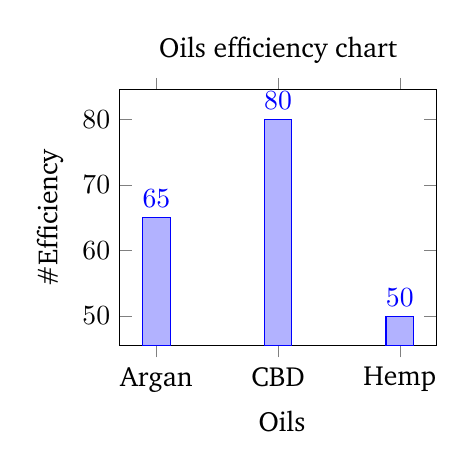
\begin{tikzpicture}  
\begin{axis}  
[  
    title=Oils efficiency chart, 
    ybar,  
    enlargelimits=0.15,  
    ylabel={\#Efficiency},   
    xlabel={\ Oils},  
    symbolic x coords={Argan, CBD, Hemp},  
    xtick=data,  
     nodes near coords,   
    nodes near coords align={vertical},  
    ]  
\addplot coordinates {(Argan,65) (CBD,80) (Hemp,50) };  
\end{axis}  
\end{tikzpicture}

     \end{frame}
    
    \begin{frame}{CBD skin benefits}

\begin{alertblock}{Important to know}
This cannabidiol comes with a plethora of astounding benefits
\end{alertblock}

\begin{block}{For instance:}
\begin{itemize}
 \item<1-> highly \alert{anti-inflammatory}
 \item<1-> reduces irritation and redness
 \item<1-> soothes psoriasis and slows down aging signs
 \item<1-> antioxidant properties
\end{itemize}
\end{block}
    
    \end{frame}

    \begin{frame}{How to use it with your skincare}
Incorporating CBD into your skincare is a great idea. Maybe you’re looking for extra protection against free radicals and oxidative stress. 

\begin{center}
\begin{table}[h!]
\centering
 \begin{tabular}{||c c||} 
 \hline
Skincare desire & Where to add \\ [0.5ex] 
 \hline\hline
 Glow skin & Add to usual cream \\ 
 \hline
 Prevent aging & Add to sunscreen  \\
 \hline
 More nutrition & Add to serum \\ [1ex]
 \hline
 \end{tabular}
\end{table}
\end{center}
\begin{alertblock}{Reminder!}
It is extremely necessary to apply strong SPF cream every day. What is more important, you should apply it even in winter.
\end{alertblock}
        
    \end{frame}

 
\end{document}
